\documentclass[12pt]{article}
\usepackage{amsmath,amssymb}
\usepackage[margin=1in]{geometry}
\usepackage[T1]{fontenc}
\usepackage{tikz}
\usetikzlibrary{arrows.meta,calc,backgrounds,positioning}
\usepackage{graphicx}\graphicspath{{figures/pdf/}{../figures/pdf/}}   % the figure suite, compiled from the repository root or from docs/

\usepackage[font=small,labelfont=bf]{caption}
\usepackage[section]{placeins}
\usepackage{needspace}
\usepackage{etoolbox}
\usepackage{array}
\usepackage{longtable}
% headings end with a period (author, 2026-10-04); the period is set by the format, not the title text, so bookmarks stay clean
\usepackage{titlesec}
\newcommand{\addperiod}[1]{#1.}
\titleformat{\section}{\normalfont\Large\bfseries}{\thesection}{1em}{\addperiod}
\titleformat{name=\section,numberless}{\normalfont\Large\bfseries}{}{0pt}{\addperiod}
\titleformat{\subsection}{\normalfont\large\bfseries}{\thesubsection}{1em}{\addperiod}
% structure: the four parts are roman-numbered sections, the twelve sections are subsections numbered 1-12 straight through
\renewcommand{\thesection}{\Roman{section}}
\counterwithout{subsection}{section}
\renewcommand{\thesubsection}{\arabic{subsection}}
% floats: a plate shares its page with the prose unless it needs the whole page (figure 5, placed [p])
\renewcommand{\topfraction}{.9}\renewcommand{\bottomfraction}{.6}\renewcommand{\textfraction}{.08}\renewcommand{\floatpagefraction}{.85}
\usepackage[hidelinks]{hyperref}

\AtBeginEnvironment{itemize}{\setlength{\itemsep}{3pt}\setlength{\parskip}{0pt}}
\setlength{\textfloatsep}{12pt plus 2pt minus 2pt}
\setlength{\intextsep}{12pt plus 2pt minus 2pt}

\title{Quantum State Spaces of Nonrigid\\ Molecules and their Complexes}
\author{Isaac AshLind}
\date{}

\newcommand{\R}{\mathbb{R}}
\newcommand{\hilb}{\mathcal{H}}
\newcommand{\hamb}{\mathcal{H}_{\mathrm{amb}}}
\newcommand{\conf}{\mathcal{C}}
\newcommand{\spin}{\mathcal{H}_{\mathrm{spin}}}
\newcommand{\act}{\mathbin{\cdot}}
\newcommand{\stat}{\chi_{\mathrm{stat}}}
\newcommand{\parity}{\chi_{\varepsilon}}
% notation (approved 2026-10-04): coordinate arrays bold, abstract operators sans serif, chart density j_varphi
\newcommand{\X}{\mathbf{X}}                 % configuration matrix; \X_0 the reference
\newcommand{\Pmat}[1]{\mathbf{P}_{#1}}      % signed right-action matrix
\newcommand{\Rmat}{\mathbf{R}}              % rotation matrix: \Rmat(r), \Rmat_h, \Rmat_z(\omega)
\newcommand{\Uop}[1]{\mathsf{U}_{#1}}       % spatial action operator
\newcommand{\Pproj}[1]{\mathsf{P}_{#1}}     % isotypic projector
\newcommand{\jdens}{j_\varphi}              % positive chart density

\begin{document}
\maketitle

\begin{center}
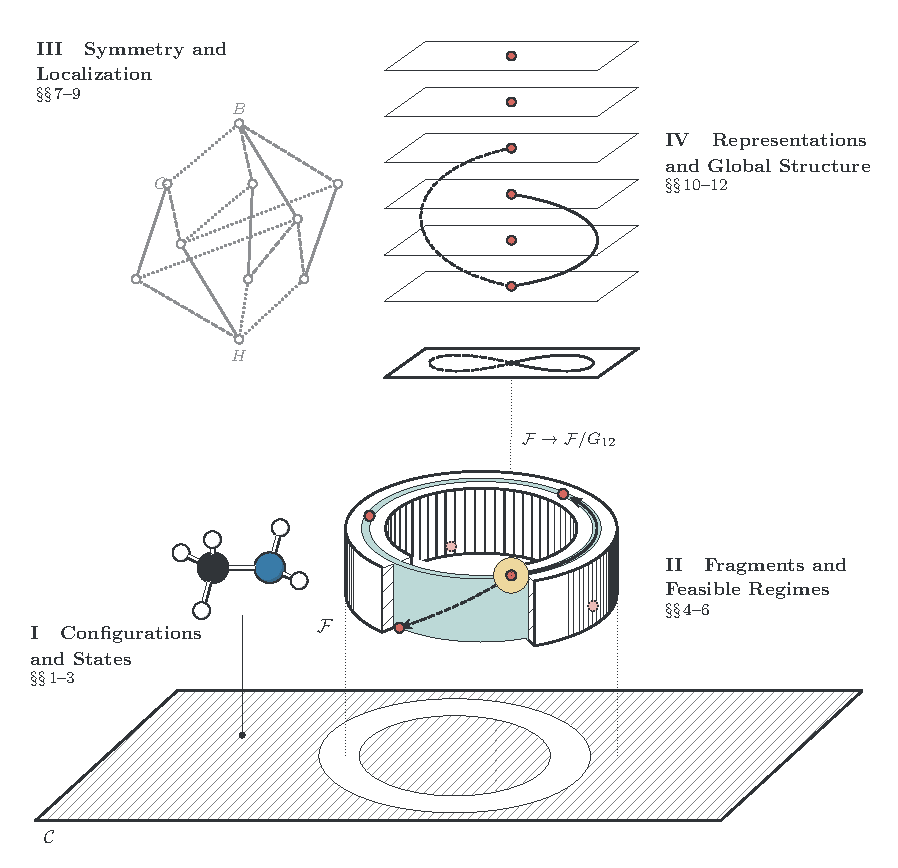
\includegraphics[width=\linewidth]{fig00-guide}\\[6pt]
{\small Guide to the paper.}
\end{center}
\clearpage


\section{Configurations and States}
\subsection{Configuration Space}

Consider $N$ labeled nuclei in Euclidean space. 
Take
the \emph{configuration space} to be the set of all linear
maps $\X: \R^N \to\R^3$ that place the center of mass
at the origin.
In a Cartesian basis, represent $\X$ by a $3\times N$ matrix whose $i$th column is the position of nucleus $i$
\[
\X=
\begin{pmatrix}
    x_1 & x_2 & \cdots & x_N \\
    y_1 & y_2 & \cdots & y_N \\
    z_1 & z_2 & \cdots & z_N
\end{pmatrix}.
\]
The column vector $\mathbf m=(m_1,\ldots,m_N)^{\mathsf T}$
contains the nuclear masses. The centered configuration
space is
\[
\conf
=
\left\{
\X\in\hom(\R^N,\R^3):\X\mathbf m=0
\right\},
\qquad
\dim\conf=3N-3.
\]

The nuclei are sorted into types by their charge, mass,
and spin, with like nuclei permutable. We also allow global
inversion. For types indexed by $\alpha$, each having
multiplicity $n_\alpha$, the overall permutation and
inversion group\footnote{The complete nuclear
permutation--inversion (CNPI) group
\cite{BunkerEtAl1997}; see also Longuet-Higgins
\cite{LonguetHiggins1963}.} is taken as
\[
S=\left(\prod_\alpha S_{n_\alpha}\right)
\times\{E,E^*\}.
\]

The inversion group $\{E,E^*\}$ is isomorphic to $C_2$.
We adopt the molecular literature's convention where
a star indicates inversion. Each element $s\in S$ is
therefore a permutation $\sigma$ or a
permutation--inversion $\sigma^*$.

As matrices, the $\X\in\conf$ form a vector space on which
permutations act by multiplication from the right
\[
s\act\X=\X\Pmat{s},
\qquad
\Pmat{\sigma^*}=-\Pmat{\sigma}.
\]
Here $\Pmat{\sigma}$ reorders the columns according to
\[
\sigma\act(\mathbf x_1,\ldots, \mathbf x_N)
=
(\mathbf x_{\sigma^{-1}(1)},\ldots,\mathbf x_{\sigma^{-1}(N)}).
\]
With this convention,
\[
s\act(t\act\X)
=(\X\Pmat{t})\Pmat{s}
=\X\Pmat{t}\Pmat{s}
=(st)\act\X.
\]
The matrices satisfy $\Pmat{st}=\Pmat{t}\Pmat{s}$. Multiplication by
these matrices on the right therefore defines a left
action of $S$ on $\conf$.

We can also act on $\X$ from the left with rotations
$r\in SO(3)$ via $3\times3$ rotation matrices $\Rmat(r)$
\[
r\act\X=\Rmat(r)\X.
\]
The actions commute by associativity
\[
r\act(s\act\X)=\Rmat(r)\X\Pmat{s}=s\act(r\act\X).
\]
We drop the dots when the action is understood.

\begin{figure}[tb]
\centering
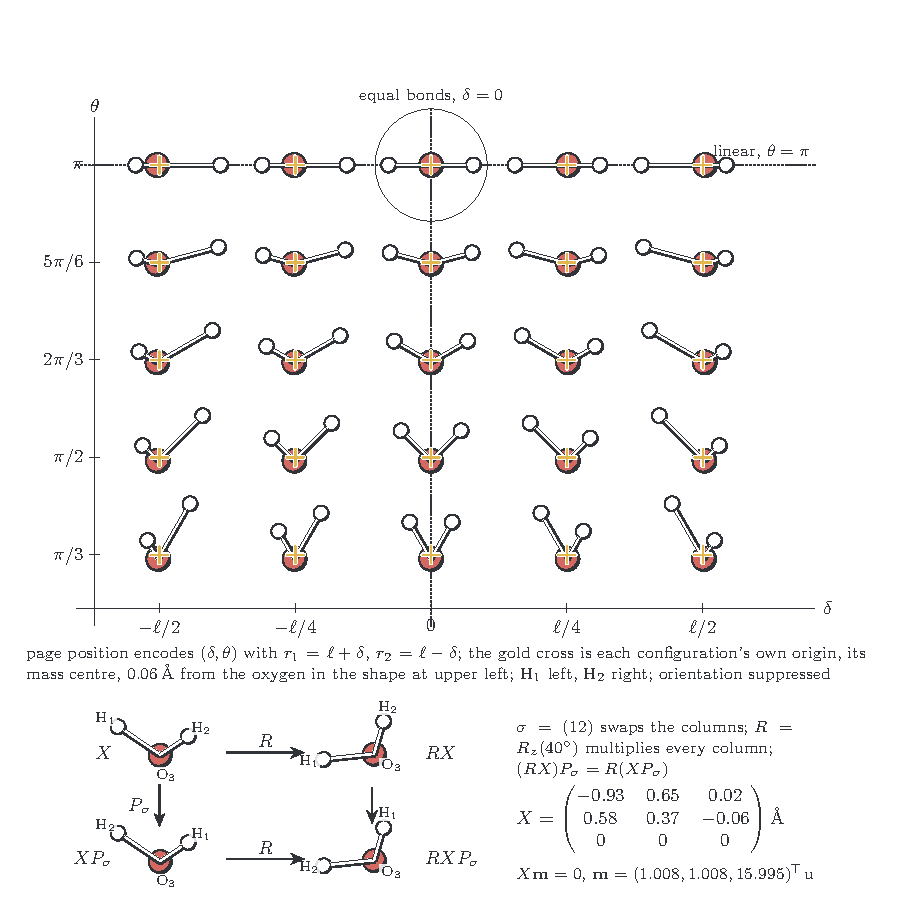
\includegraphics[width=\linewidth]{fig01-configuration-space}
\caption{(author caption; see docs/caption-notes.md)}\label{fig:1}
\end{figure}

\subsection{Ambient Hilbert Space}

The \emph{ambient Hilbert space} for our configuration space,
including the spin of the nuclei, is
\[
\hamb=L^2(\conf)\otimes\spin,
\qquad
\spin=\bigotimes_{i=1}^{N}\mathbb C^{2I_i+1}.
\]
Here $L^2(\conf)$ uses the translation-invariant volume
measure $d\X$ up to normalization.
The $i$th nucleus has spin number $I_i$, and its
spin vectors lie in $\mathbb C^{2I_i+1}$. A general vector
in $\spin$ is a linear combination of products
$\xi_1\otimes\cdots\otimes\xi_N$, with factors ordered
by nuclear label.

The group $S$ permutes like-nucleus spin factors in the
same order as the configuration columns, with inversion
acting trivially
\[
s\act(\xi_1\otimes\cdots\otimes\xi_N)
=
\xi_{\sigma^{-1}(1)}\otimes\cdots\otimes
\xi_{\sigma^{-1}(N)},
\]
where $\sigma$ is the permutation underlying $s$.
The action extends linearly to all spin vectors.

A wavefunction is a square-integrable map
\[
\Psi:\conf\to\spin,
\qquad
\|\Psi\|^2
=
\int_{\conf}\|\Psi(\X)\|_{\spin}^2\,d\X<\infty.
\]
For example, if $\xi,\zeta\in\spin$ are orthonormal and
$\Psi(\X)=a(\X)\xi+b(\X)\zeta$, then
\[
\|\Psi(\X)\|_{\spin}^2=|a(\X)|^2+|b(\X)|^2,
\qquad
\|\Psi\|^2
=
\int_{\conf}\bigl(|a(\X)|^2+|b(\X)|^2\bigr)\,d\X.
\]

As in $L^2(\R^n)$, we identify wavefunctions whose
difference has zero norm
\[
\Psi\sim\Phi
\quad\Longleftrightarrow\quad
\int_{\conf}
\|\Psi(\X)-\Phi(\X)\|_{\spin}^2\,d\X=0.
\]

\begin{figure}[tb]
\centering
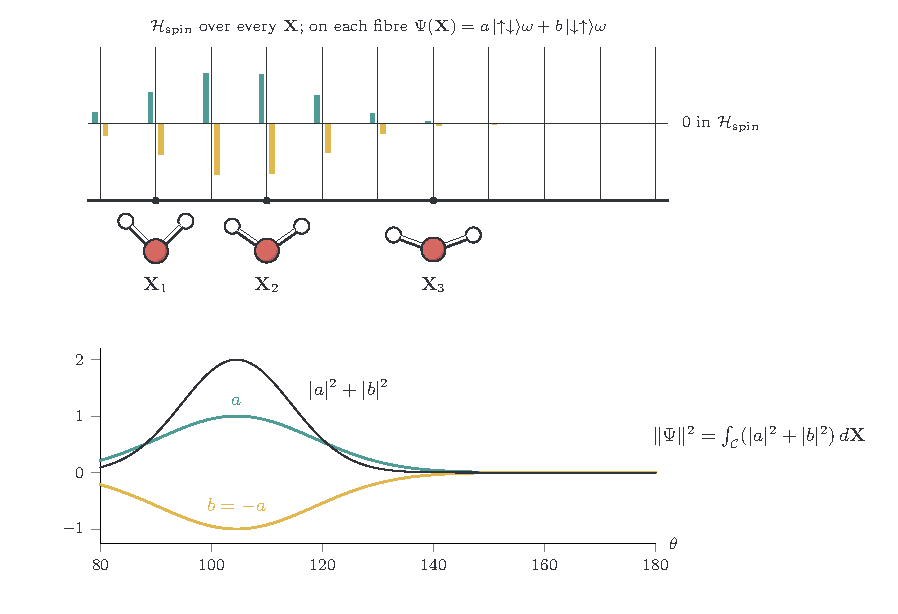
\includegraphics[width=\linewidth]{fig02-ambient-hilbert-space}
\caption{(author caption; see docs/caption-notes.md)}\label{fig:2}
\end{figure}

\subsection{Physical Hilbert Space}

Exchange statistics select the \emph{physical Hilbert
space} $\hilb\subseteq\hamb$.

Inversion imposes no additional exchange-statistics
constraint, so we pass to $S/\langle E^*\rangle$,
identifying each coset $\{\sigma,\sigma^*\}$ with its
underlying permutation $\sigma$. Let $\sigma_\alpha$
be its restriction to nuclei of type $\alpha$, with
spin number $I_\alpha$. The statistics character is
\[
\stat(\sigma)
=
\prod_\alpha
\bigl(\operatorname{sgn}\sigma_\alpha\bigr)^{2I_\alpha}.
\]
Recall that $\Psi(\X)$ is a spin vector and $\sigma$ permutes
spin factors. Write
$(\Psi\circ\sigma)(\X)=\Psi(\sigma\X)$ and
$(\sigma\cdot\Psi)(\X)=\sigma\cdot\Psi(\X)$. Using the equivalence relation defined above,
the physical Hilbert space is
\[
\hilb
=
\left\{
\Psi\in\hamb
:
\Psi\circ\sigma
\sim
\stat(\sigma)\,\sigma\act\Psi,
\quad\forall\,\sigma\in S/\langle E^*\rangle
\right\}.
\]
In words, the physical wavefunctions are those which respect
exchange statistics under permutations in the configuration
space, with the spin factors reorganized accordingly.

The parity sectors of the physical Hilbert space are
\[
\hilb_\pm=\{\Psi\in\hilb:\Psi\circ E^*\sim\pm\Psi\},
\]
where $(\Psi\circ E^*)(\X)=\Psi(-\X)$.
They give the orthogonal decomposition
\[
\hilb=\hilb_+\oplus\hilb_-,
\qquad
\Psi=\Psi_++\Psi_-,
\qquad
\Psi_\pm(\X)=\frac12\bigl(\Psi(\X)\pm\Psi(-\X)\bigr).
\]
Extend $\stat$ to $S$ by ignoring the star, and define
the parity characters by
\[
\chi_\pm(\sigma)=1,
\qquad
\chi_\pm(\sigma^*)=\pm1.
\]
A physical wavefunction of parity $\pm$ then obeys
\[
\Psi_\pm\circ s
\sim
\stat(s)\chi_\pm(s)\,s\cdot\Psi_\pm,
\qquad\forall s\in S.
\]
Here composition acts on the configuration argument,
while $s\cdot\Psi_\pm$ acts on the spin factors.

\begin{figure}[tb]
\centering
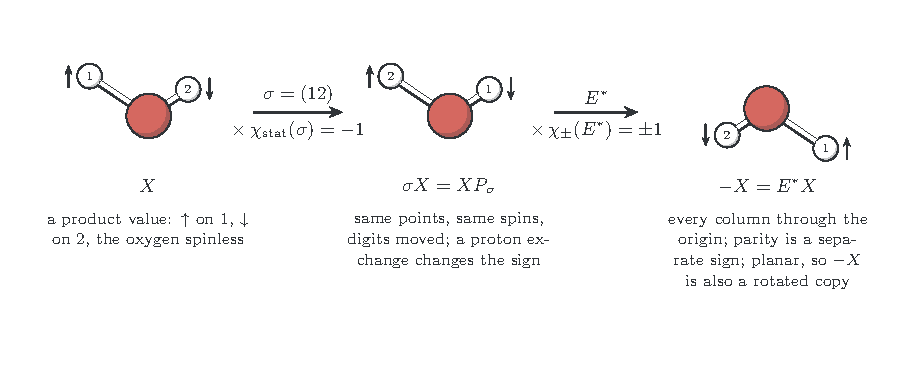
\includegraphics[width=\linewidth]{fig03-physical-hilbert-space}
\caption{(author caption; see docs/caption-notes.md)}\label{fig:3}
\end{figure}


\section{Fragments and Feasible Regimes}
\subsection{Molecules, Fragments, and Complexes}
\begin{itemize}
\item Partition the nuclei into fragments. One molecule is the
one-fragment case. Relative fragment positions and orientations remain in $\conf$.
\item For KRb + KRb, label potassium $1,2$ and rubidium $3,4$.
\end{itemize}
\[
\mathrm{KRb}+\mathrm{KRb}
\longrightarrow\mathrm K_2\mathrm{Rb}_2
\longrightarrow\mathrm K_2+\mathrm{Rb}_2,
\qquad S=\langle(12),(34),E^*\rangle\cong C_2^3.
\]
\[
G_{\mathrm{in}}=\langle(12)(34),E^*\rangle,
\qquad G_{\mathrm K}=\langle(12),E^*\rangle,
\qquad G_{\mathrm{Rb}}=\langle(34),E^*\rangle.
\]
\begin{itemize}
\item Each channel group has order $4$. Any two generate $S$.
Separate group inclusion from physical accessibility.
\item For $^{40}\mathrm K{}^{87}\mathrm{Rb}$, experiment finds
near-conservation of nuclear spin and corresponding product rotational
parities.\footnote{Hu et al.\ \cite{HuEtAl2021}.}
Symmetry gives allowed sectors, not yields.
\item Choose a reference geometry to count versions.
\end{itemize}

\begin{figure}[tb]
\centering
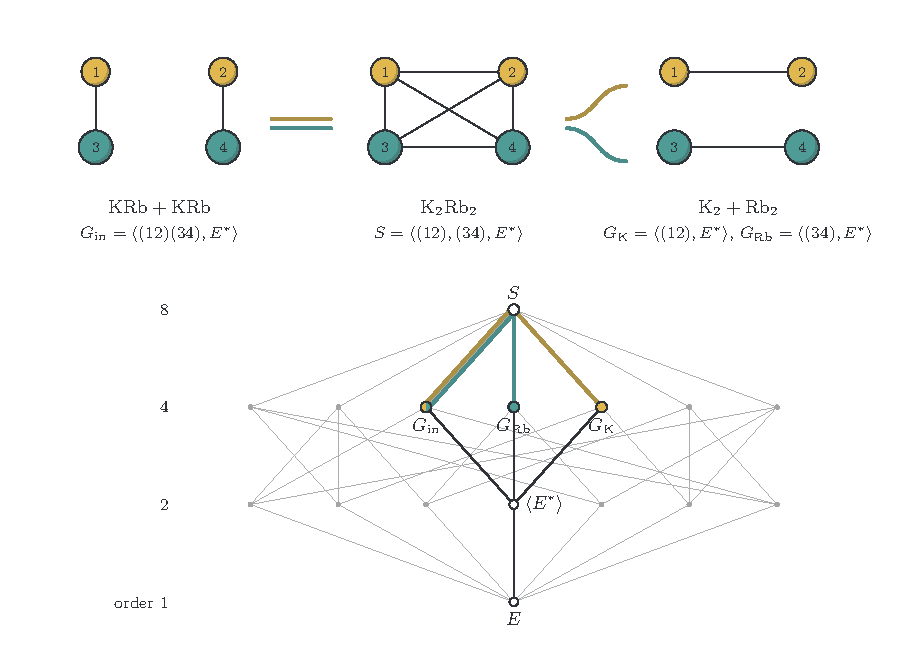
\includegraphics[width=\linewidth]{fig04-molecules-fragments-complexes}
\caption{(author caption; see docs/caption-notes.md)}\label{fig:4}
\end{figure}

\subsection{Symmetry Groups and Versions}
\label{sec:feasible-regimes}

The construction so far accommodates all possible
arrangements of nuclei without imposing energetic or
experimental restrictions. Experimental resolution informs the choice of a feasible
regime with a group $G\leq S$ of feasible operations. For a given configuration $\X$,
there is a natural minimal symmetry $H$ consisting of the
permutation--inversions equivalent to rotations in $SO(3)$. By looking at the subgroup lattice for $H\leq G\leq S$
along with a reference configuration and chosen paths,
we can carve out the shapes of feasible regimes and
their symmetries without first specifying a potential.
This is a kinematic model. Which
regimes are accessible in practice is left to experiment.

Choose a reference configuration $\X_0$ and look at its orbit
under rigid rotations,
\[
SO(3)\X_0=\{r\X_0:r\in SO(3)\}.
\]
Its point group is the subgroup
\[
H
=
\{h\in S:h\X_0\in SO(3)\X_0\}.
\]
The point group $H$ stabilizes the rotational orbit of $\X_0$.
Thus, for every $h\in H$, there is a rotation $\Rmat_h\in SO(3)$
such that
\[
h\X_0=\Rmat_h\X_0.
\]
For nonlinear $\X_0$, this rotation is unique. The rotational
orbit $SO(3)\X_0$ describes the rigid reference, and $G=H$ is
the minimal feasible regime.

A rearrangement is described by a continuous path
\[
\gamma:[0,1]\to\conf
\]
beginning at $\X_0$ and ending at a rotated,
permutation--inverted copy of $\X_0$,
\[
\gamma(0)=\X_0,
\qquad
\gamma(1)=rs\X_0,
\]
for some $r\in SO(3)$ and $s\in S$. The motion is
nonrigid if the path leaves $SO(3)\X_0$.

If the resolved motions correspond to
$s_1,\ldots,s_k\in S$, they generate the feasible group
\[
G=\langle H,s_1,\ldots,s_k\rangle,
\qquad
H\leq G\leq S.
\]
The cosets $G/H$ are the versions\footnote{The term
\emph{version} follows Bunker and Jensen
\cite{BunkerJensen1998}; the full set of versions is $S/H$,
while $G/H$ gives those accessible within the regime.}
accessible within the regime.

Adding an operation $s$ moves from $G$ to $\langle G,s\rangle$.

\begin{itemize}
\item Take CH$_3$NH$_2$ with five hydrogens of the same isotope.
Label methyl hydrogens $1,2,3$, amino hydrogens $4,5$, carbon $6$, and nitrogen $7$.
\item Choose the reference mirror plane through $1,6,7$, exchanging
$2$ with $3$ and $4$ with $5$.
\end{itemize}
\[
S=S_5\times\{E,E^*\},\qquad |S|=240,
\qquad H=\langle b\rangle,\qquad b=(23)(45)^*.
\]
\begin{itemize}
\item Keeping bonds restricts the candidates to $[H,B]$.
Here $S_A$ permutes the labels in $A$.
\end{itemize}
\[
B=(S_{\{1,2,3\}}\times S_{\{4,5\}})\times\{E,E^*\},
\qquad |B|=24,
\qquad t=(123),\quad u=(45).
\]
\[
G_6=\langle H,t\rangle,\qquad |G_6/H|=3,
\qquad G_{12}=\langle H,t,u\rangle,\qquad |G_{12}/H|=6.
\]
\begin{itemize}
\item Above $G_6$, adding $u$, $E^*$, or $u^*$ gives three order-$12$
candidates. Any two extensions generate $B$.
\item Microwave and far-infrared spectra resolve torsion and inversion
in the $G_{12}$ regime.\footnote{Ilyushin et al.\
\cite{IlyushinEtAl2005} and Kr\k{e}glewski~\cite{Kreglewski2009}.}
The amino inversion includes a corrective $60^\circ$ methyl turn,
represented by $tu$.\footnote{Kleiner and Hougen~\cite{KleinerHougen2015}.}
\item Comparing the candidates through their species and spin weights is
the intended test; Sections~\ref{sec:species} and~\ref{sec:weights} carry
it out for $G_6$.
The full interval $[H,S]$ has $36$ subgroups, compared with $10$ in $[H,B]$.
\end{itemize}

\begin{figure}[p]
\centering
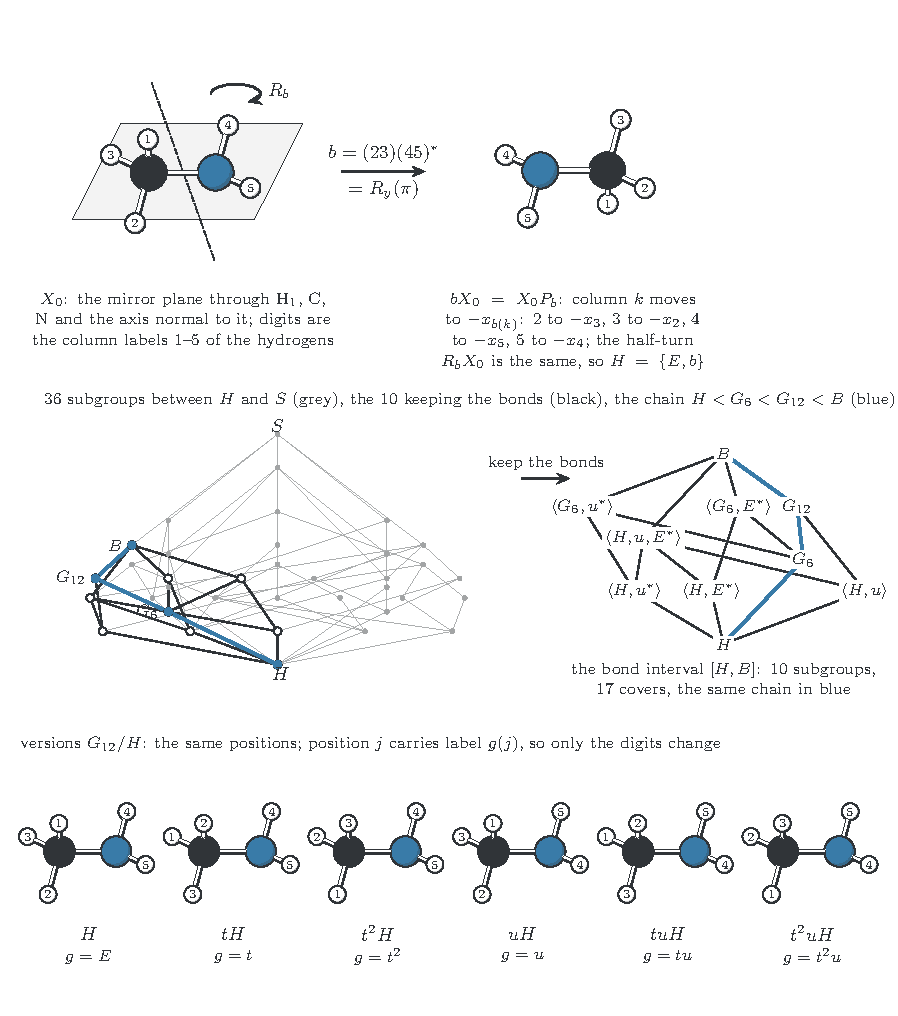
\includegraphics[width=\linewidth]{fig05-symmetry-groups-versions}
\caption{(author caption; see docs/caption-notes.md)}\label{fig:5}
\end{figure}

\subsection{Feasible Configuration Space}
\label{sec:feasible-space}
\begin{itemize}
\item Sweep chosen rearrangement paths through rotations and $G$.
Thicken in the normal directions to obtain a connected region
$\mathcal F\subseteq\conf$.
\item Require $s\mathcal F=\mathcal F$ for $s\in G$ and
$s\mathcal F\cap\mathcal F=\varnothing$ otherwise.
The copies are indexed by $S/G$, with $|G/H|$ reference versions in each.
\end{itemize}
\[
S/H\longrightarrow S/G,\qquad sH\longmapsto sG.
\]
\begin{itemize}
\item For methylamine's $G_{12}$ regime, sweep the torsional circle
along the umbrella coordinate. Picture a short tube $S^1\times[-1,1]$,
thickened by normal displacements, with orientations over each shape.
\item The illustrated model assumes the product structure, connectedness,
and separation. The rigid specialization is recovered by freezing internal
shape and excluding rearrangements; see the closing box in
Section~\ref{sec:momentum}.
\end{itemize}
\begin{itemize}
\item For an exact support restriction, use the whole symmetry-related union.
\end{itemize}
\[
\hilb_{\mathcal F}
=\left\{\Psi\in\hilb:
\Psi=0\text{ a.e. outside }\bigcup_{s\in S}s\mathcal F\right\}.
\]
\begin{itemize}
\item For open regions, compactly supported smooth packets, combined
with spin and projected onto exchange statistics, span this space densely.
Gaussians retain tails.
\item Nested regions give nested state spaces. Group inclusion alone
does not specify geometric inclusion.
\end{itemize}

\begin{figure}[tb]
\centering
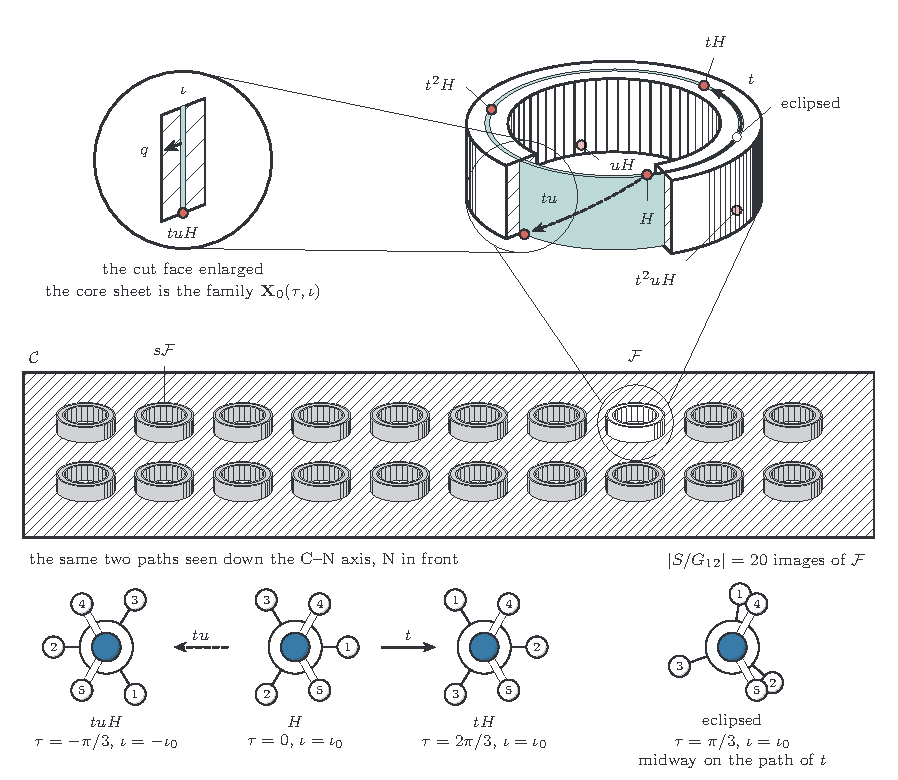
\includegraphics[width=\linewidth]{fig06-feasible-configuration-space}
\caption{(author caption; see docs/caption-notes.md)}\label{fig:6}
\end{figure}


\section{Symmetry and Localization}
\subsection{Symmetry Species}
\label{sec:species}
\begin{itemize}
\item The irreducible representations of $G$ are its \emph{species}.
Pair spatial species with nuclear spin and compute spin weights.
\item Project a spatial state onto each species. Write
$\chi_\Gamma=\operatorname{tr}\Gamma$ and $d_\Gamma=\dim\Gamma$.
The projector retains all copies of that species.
\end{itemize}
\[
(\Uop{g}f)(\X)=f(g^{-1}\X),\qquad
\Pproj{\Gamma}=\frac{d_\Gamma}{|G|}
\sum_{g\in G}\chi_\Gamma(g^{-1})\,\Uop{g}.
\]
\[
w_\Gamma(f)=\frac{\|\Pproj{\Gamma} f\|^2}{\|f\|^2},
\qquad \sum_\Gamma w_\Gamma(f)=1,\qquad f\ne0.
\]
\begin{itemize}
\item Choose states at one version, specify their $H$ action, and induce
over $G/H$. Start with a local vibrational ground state at fixed
rotational angular momentum.
\item One scalar state fixed by $H$ gives methylamine's three torsional
version states.
\end{itemize}
\[
\mathbb C[G_6/H]\cong\mathrm A_1\oplus\mathrm E.
\]
\begin{itemize}
\item Follow species across subgroup inclusions.
\item Use double cosets to organize connections between versions.
\item For complexes, induce incoming channel states and restrict to
product groups.
\end{itemize}

\begin{figure}[tb]
\centering
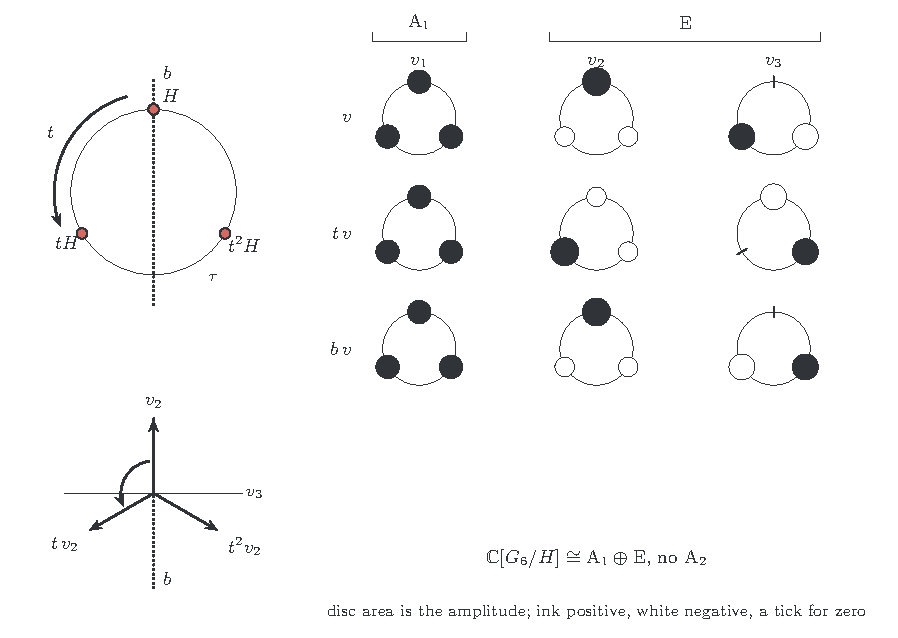
\includegraphics[width=\linewidth]{fig07-symmetry-species}
\caption{(author caption; see docs/caption-notes.md)}\label{fig:7}
\end{figure}

\subsection{Nuclear Spin Weights}
\label{sec:weights}
\begin{itemize}
\item Restrict the nuclear-spin action of $S$ to the feasible group $G$.
Inversion acts trivially on spin, so only the permutation part of $G$ acts.
\item Decompose $\spin$ under $G$ into species, counting copies rather
than dimensions. For the five protons of methylamine under $G_6$,
\end{itemize}
\[
\spin\cong 12\,\mathrm A_1\oplus 4\,\mathrm A_2\oplus 8\,\mathrm E,
\qquad 12+4+2\cdot 8=32,
\]
\begin{itemize}
\item so the eight copies of $\mathrm E$ fill sixteen of the thirty-two
dimensions.
\item A spatial state of species $\Gamma$ and parity $\pm$ pairs with the
spin species $\Gamma'$ for which $\Gamma\otimes\Gamma'$ contains the
character $\stat\chi_\pm$ of the physical-state condition. On $G_6$,
$\stat=1$: even parity pairs each species with itself; odd parity exchanges
$\mathrm A_1$ with $\mathrm A_2$ and keeps $\mathrm E$.
\item The weight of a spatial level is the number of physical states it
carries, one for each copy of its partner species (Figure~\ref{fig:8}):
\end{itemize}
\begin{center}\small
\begin{tabular}{lcc}
\hline
spatial species & even parity & odd parity\\
\hline
$\mathrm A_1$ & 12 & 4\\
$\mathrm A_2$ & 4 & 12\\
$\mathrm E$ & 8 & 8\\
\hline
\end{tabular}
\end{center}

\begin{figure}[tb]
\centering
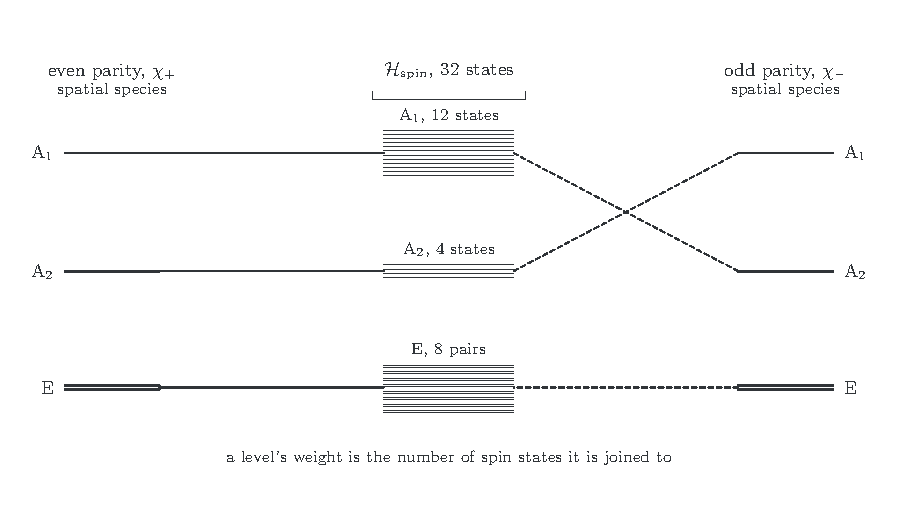
\includegraphics[width=\linewidth]{fig08-nuclear-spin-weights}
\caption{(author caption; see docs/caption-notes.md)}\label{fig:8}
\end{figure}

\subsection{Localized States}
\label{sec:localized-states}
\begin{itemize}
\item In $G_6$, choose a normalized real scalar packet $g_0$, fixed
by $H$ and localized near the reference rotational orbit.
Its translates sit at $H,tH,t^2H$.
\end{itemize}
\[
g_j(\X)=g_0(t^{-j}\X),\qquad j=0,1,2.
\]
\begin{itemize}
\item All pairwise overlaps equal $c=\langle g_0,g_1\rangle$.
The squared spatial projection shares of $g_0$ are
\end{itemize}
\[
w_{\mathrm A_1}=\frac{1+2c}{3},\qquad
w_{\mathrm E}=\frac{2(1-c)}{3},\qquad w_{\mathrm A_2}=0.
\]
\begin{itemize}
\item Independent packets span $\mathrm A_1\oplus\mathrm E$.
For a planar illustration, take equal Gaussians of position variance
$\Delta^2$ on an equilateral triangle of side $d$.
\end{itemize}
\[
c=\exp\!\left(-\frac{d^2}{8\Delta^2}\right).
\]
\begin{itemize}
\item Add $u$-related packets for the six versions in $G_{12}/H$.
Resolve the $u$ action through sums and differences.
\item Pair with spin and impose the feasible support restriction
of Section~\ref{sec:feasible-space}, when required.
\item Treat symmetry-enforced nodes with the required pointwise regularity.
\end{itemize}

\begin{figure}[tb]
\centering
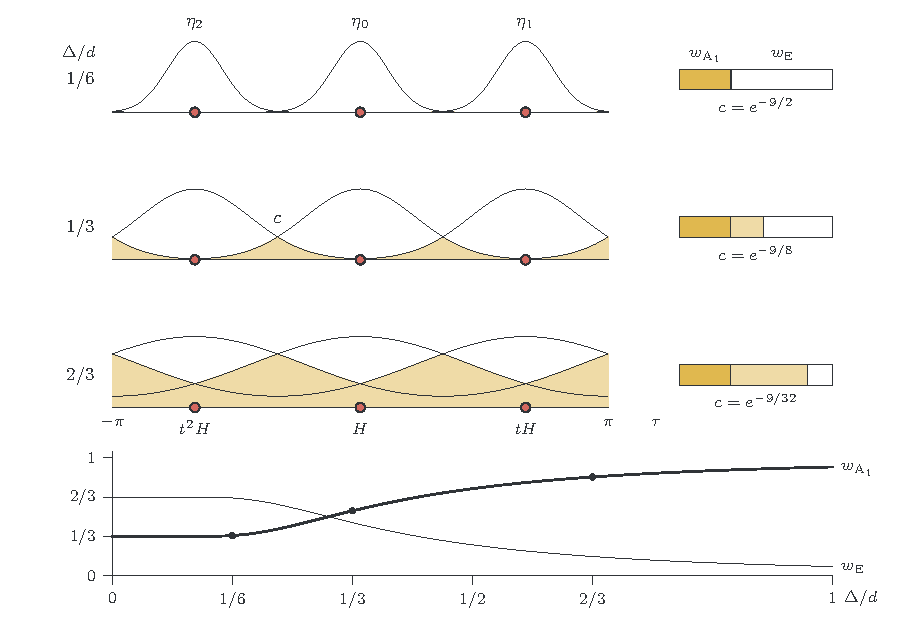
\includegraphics[width=\linewidth]{fig09-localized-states}
\caption{(author caption; see docs/caption-notes.md)}\label{fig:9}
\end{figure}


\section{Representations and Global Structure}
\subsection{Position Representation}
\label{sec:position-coordinates}
\begin{itemize}
\item Choose a body frame and a mass-orthogonal normal frame $\mathbf e_\alpha(a)$.
Use $r$ for orientation, $a$ for internal shape, and $q$ for normal coordinates.
\end{itemize}
\[
\varphi(r,a,q)=\Rmat(r)\left(\X_0(a)+\sum_{\alpha=1}^{n_q}q_\alpha\mathbf e_\alpha(a)\right),
\qquad\psi(r,a,q)=\Psi\bigl(\varphi(r,a,q)\bigr).
\]
\begin{itemize}
\item On a regular chart, pull back the configuration measure.
Here $dr$ is normalized Haar measure and $\jdens$ is the chart density.
\end{itemize}
\[
d\mu=\jdens(a,q)\,dr\,da\,dq,
\qquad
\|\Psi\|_{\varphi(\mathcal U)}^2
=\int_{\mathcal U}\|\psi(r,a,q)\|_{\spin}^2\,d\mu.
\]
\begin{itemize}
\item The generalized states $|r,a,q\rangle$ resolve the chart identity with $d\mu$.
\item Write $x=(r,a,q)$. Carry each configuration action through the
source and target charts. For $s\in S$, solve for $x'=T_sx$.
\end{itemize}
\[
T_s=\varphi_{\mathrm{target}}^{-1}\circ s\circ\varphi_{\mathrm{source}},
\]
\begin{itemize}
\item On a symmetry-invariant reference family, first find the new
shape $a'$ and compensating rotation $\mathbf A_s(a)$. Expand the transformed
normal frame in the target frame to obtain $\mathbf M_s(a)$.
\end{itemize}
\[
\begin{aligned}
\X_0(a)\Pmat{s}&=\mathbf A_s(a)\X_0(a'),\\
\mathbf e_\alpha(a)\Pmat{s}&=\mathbf A_s(a)\sum_\beta\mathbf e_\beta(a')\,[\mathbf M_s(a)]_{\beta\alpha},\\
T_s(r,a,q)&=\bigl(r\mathbf A_s(a),a',\mathbf M_s(a)q\bigr).
\end{aligned}
\]
\begin{itemize}
\item Here $\mathbf A_s(a)$ is the matrix of a rotation, and $r\mathbf A_s(a)$
denotes the orientation whose matrix is $\Rmat(r)\mathbf A_s(a)$; the same
reading applies to $r\Rmat_z(\omega)$ below.
\item This is exact on the normal chart. Finding $a'$ uses the chosen
shape coordinates, and the normal-frame expansion is linear algebra.
\item A lab rotation $r_0$ gives $T_{r_0}(r,a,q)=(r_0r,a,q)$.
The induced spatial operator is the inverse pullback. Permuting the
spin factors gives the physical-state condition.
\end{itemize}
\[
(\Uop{s}\psi)(x)=\psi(T_s^{-1}x),\qquad \Uop{s}|x\rangle=|T_sx\rangle.
\]
\[
\psi(T_\sigma x)\sim\stat(\sigma)\,\sigma\act\psi(x).
\]
\begin{itemize}
\item With $\widetilde\psi=\jdens^{1/2}\psi$, the same operator in
the measure $dr\,da\,dq$ includes the density ratio.
\end{itemize}
\[
(\widetilde{\mathsf U}_s\widetilde\psi)(x)
=\left(\frac{\jdens(x)}{\jdens(T_s^{-1}x)}\right)^{1/2}
\widetilde\psi(T_s^{-1}x).
\]
\begin{itemize}
\item Use these formulas wherever the source and target charts apply.
Treat axial redundancy at linear configurations.
\end{itemize}

\begin{itemize}
\item For an explicit methylamine model, take the C--N axis as body $z$
and use $\iota$ for the umbrella coordinate. In a periodic body frame,
$tu$ gives a half-turn of the frame, a $-\pi/3$ torsional shift,
and $\iota\mapsto-\iota$.\footnote{One reference family places the amino
hydrogens at $(\iota,\pm b_A,z_A)$ and the methyl hydrogens at angles
$\tau-2\pi(k-1)/3$, $k=1,2,3$, at fixed radius and height about
the C--N axis. Center the whole configuration as before.}
\item Twist the body frame by $\Rmat_z(-\rho\tau)$, with $\rho$ a chosen
frame parameter; we take $\rho=\tfrac12$, the analogue for one methyl top of
the symmetric internal-axis frame used for ethane by Mellor, Yurchenko, Mant
and Jensen~\cite{MellorEtAl2019}. Retain two normal
coordinates $q_+,q_-$ chosen to transform evenly and oddly under $tu$.
These are symmetry-adapted coordinates, not vibrational eigenmodes.
\end{itemize}
\[
\omega_{tu}=\pi-\frac{\rho\pi}{3},\qquad
x=(r,\tau,\iota,q_+,q_-),
\]
\[
T_{tu}x=\bigl(r\Rmat_z(\omega_{tu}),\tau-\pi/3,-\iota,q_+,-q_-\bigr),
\]
\[
(\Uop{tu}\psi)(x)
=\psi\bigl(r\Rmat_z(-\omega_{tu}),\tau+\pi/3,-\iota,q_+,-q_-\bigr).
\]
\begin{itemize}
\item Six applications close through the seam of Section~\ref{sec:momentum}.
For proton exchange, $\stat(tu)=-1$.
\end{itemize}
\[
T_{tu}^{\,6}x
=\bigl(r\Rmat_z(-2\pi\rho),\tau-2\pi,\iota,q_+,q_-\bigr)\sim x,
\qquad \psi(T_{tu}x)\sim-(tu)\act\psi(x).
\]
\begin{itemize}
\item General normal coordinates replace the signs by matrices.
The rotational factor records the frame choice. It does not prescribe
dynamical rotational transport.
\end{itemize}

\begin{figure}[tb]
\centering
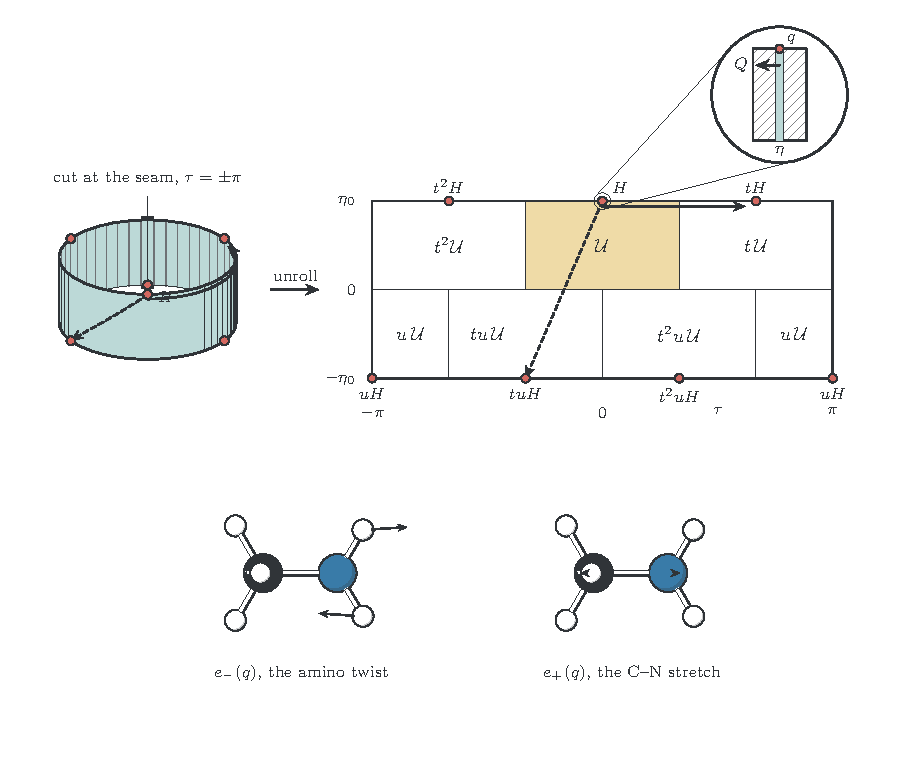
\includegraphics[width=\linewidth]{fig10-position-representation}
\caption{(author caption; see docs/caption-notes.md)}\label{fig:10}
\end{figure}

\subsection{Covering Spaces and Monodromy}
\begin{itemize}
\item Versions label rotational orbits in $G/H$. Charts give local coordinates.
\item For methylamine, choose an $H$-invariant cell $\mathcal U$ whose
translates partition $\mathcal F$ up to their walls. Glue orientations,
normal coordinates, and wavefunctions across the walls.
\end{itemize}
\[
(G_{12}\times_H\mathcal U)/{\sim}\cong\mathcal F.
\]
\begin{itemize}
\item For a free action, $\mathcal F\to\mathcal F/G$ is a covering
with deck group $G$. A lifted chart transition induced by $g$
is a local expression of its deck transformation.
\item A path $\X\to g\X$ projects to a loop. Its lift stays in one
feasible component and records the sheet change, or
\emph{monodromy}.\footnote{Hatcher~\cite{Hatcher2002}, Section 1.3.}
\item Near a free reference configuration, twelve local sheets group
in pairs within six version cells. $G_{12}/H$ is a coset set, not a group.
\end{itemize}
\[
t^3=b^2=E,\qquad btb=t^{-1},\qquad bt=t^2b\ne tb.
\]
\begin{itemize}
\item A species sees $g$ through $\Gamma(g)$, with
$\Gamma(G)\cong G/\ker\Gamma$. On $G_6$, $\mathrm A_1$ sees no change,
while $\mathrm E$ retains noncommutativity.
\item Treat fixed configurations separately; the rigid orientation
construction is recovered in the box closing
Section~\ref{sec:momentum}.\footnote{Albert et al.\ \cite{AlbertEtAlOrientation}.}
\item Distinguish chart gluing from mechanical parallel
transport.\footnote{Littlejohn and Reinsch~\cite{LittlejohnReinsch1997}.}
A Berry interpretation needs
a specified state family and connection.
\end{itemize}

\begin{figure}[tb]
\centering
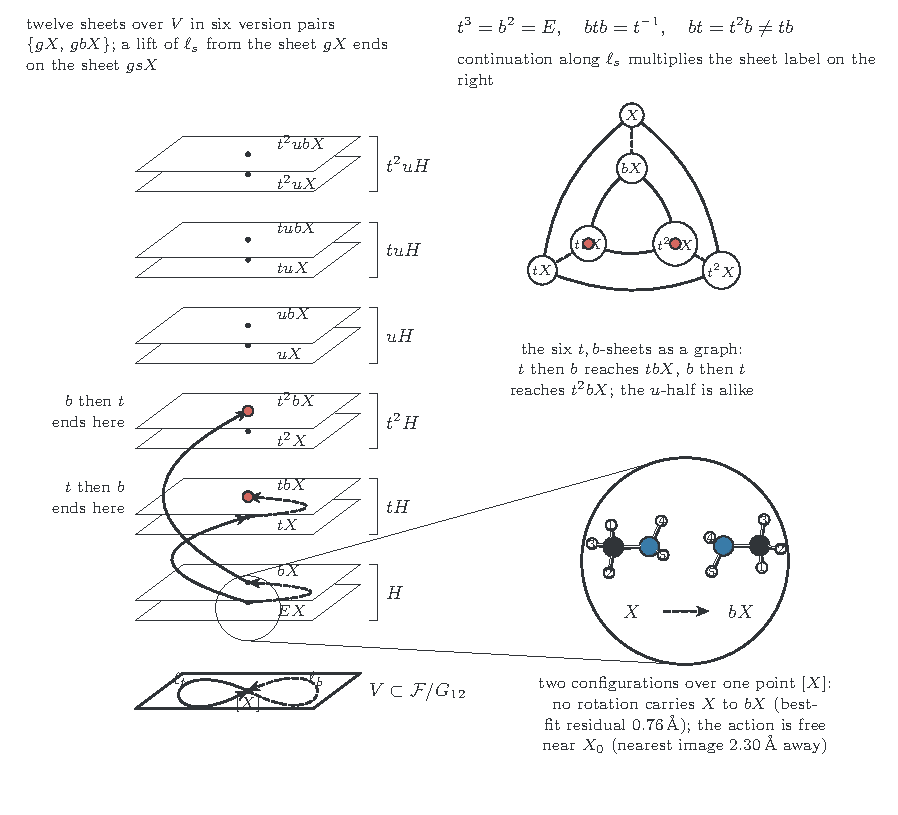
\includegraphics[width=\linewidth]{fig11-covering-spaces-monodromy}
\caption{(author caption; see docs/caption-notes.md)}\label{fig:11}
\end{figure}

\subsection{Momentum Representation}
\label{sec:momentum}
\begin{itemize}
\item Expand the same states in rotational, internal, and normal modes,
subject to the chart identifications; the example below is a reduced
torsional model, not a transform of the full torsion--umbrella model.
\item For the product model $SO(3)\times S^1\times\R^{n_q}$, with $\iota$ held
at its reference value and omitted from the product (a reduced torsional
model), absorb the density into $\widetilde\psi=\jdens^{1/2}\psi$.
Use the measure $dr\,d\tau\,dq$, denoted by the subscript $0$.
\end{itemize}
\[
\langle r,\tau,q\mid JMK,m,p\rangle_0
=\frac{\sqrt{2J+1}\,D^J_{MK}(r)\,e^{im\tau}e^{ip\cdot q/\hbar}}
{\sqrt{2\pi}\,(2\pi\hbar)^{n_q/2}}.
\]
\[
J\in\mathbb N_0,\qquad -J\le M,K\le J,\qquad m\in\mathbb Z,
\qquad p\in\R^{n_q}.
\]
\begin{itemize}
\item The coefficients $\widehat\psi_{JMKm}(p)$ are spin vectors.
Sum over $J,M,K,m$ and integrate over $p$ for the inverse transform.
No energies are assigned; the product structure is assumed here.
\item Let the body frame close with a turn while the normal frame closes on itself.
\end{itemize}
\[
(r,\tau+2\pi,q)\sim\bigl(r\Rmat_z(-2\pi\rho),\tau,q\bigr),
\qquad D^J_{MK}(r\Rmat_z(\omega))=e^{-iK\omega}D^J_{MK}(r).
\]
\[
e^{2\pi i\kappa}=e^{2\pi i\rho K},\qquad
\kappa=m+\rho K=m+\tfrac12K,\qquad m\in\mathbb Z.
\]
\begin{itemize}
\item Periodic and twisted frames give integer and shifted labels for
the same states. Include normal-frame gluing when present.
\end{itemize}
\begin{itemize}
\item For periodic scalar torsion, take $f_m(\tau)=e^{im\tau}$,
with $t:\tau\mapsto\tau+2\pi/3$ and $b:\tau\mapsto-\tau$.
\end{itemize}
\[
\Uop{g}f=f\circ g^{-1},\qquad
\Uop{t}f_m=e^{-2\pi im/3}f_m,\qquad \Uop{b}f_m=f_{-m}.
\]
\begin{itemize}
\item The species of the modes are those of Figure~\ref{fig:12}: $\mathrm A_1$
at $m=0$, an $\mathrm E$ pair when $3\nmid m$, and $\mathrm A_1\oplus\mathrm A_2$
(cosine, sine) at nonzero multiples of $3$; their spin partners follow the
rule of Section~\ref{sec:weights}. The coupled torsion and inversion of
methylamine lies outside the present example.
\end{itemize}

\begin{figure}[tb]
\centering
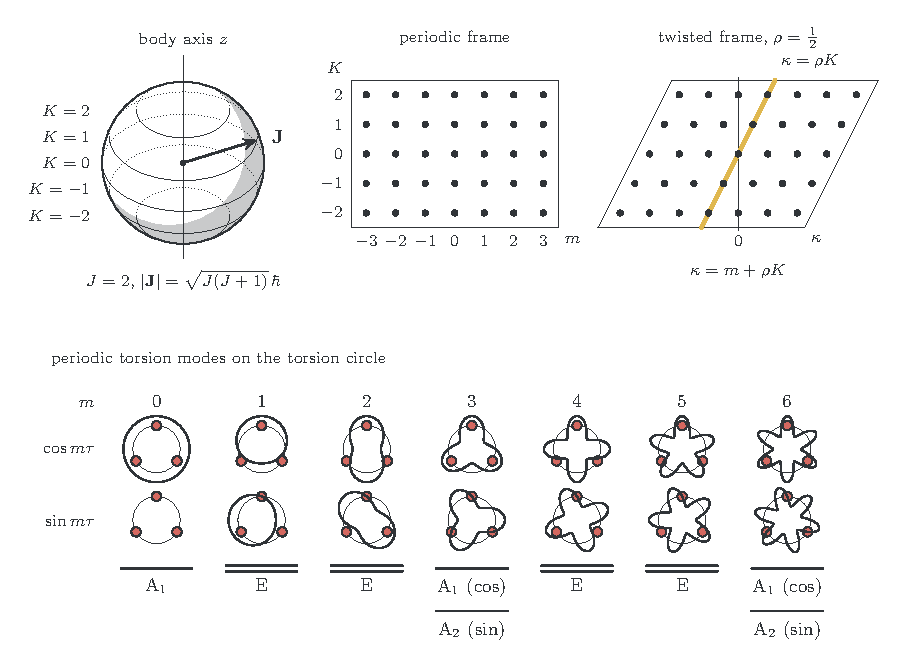
\includegraphics[width=\linewidth]{fig12-momentum-representation}
\caption{(author caption; see docs/caption-notes.md)}\label{fig:12}
\end{figure}

% ---- closing box: the rigid formulation as a kinematic specialization (author's draft, 2026-10-04; one box, kept whole)
\begingroup\setlength{\fboxsep}{7pt}\setlength{\fboxrule}{.4pt}
% the box is typeset once into a register so that its height is known: if it does not fit on the current page it
% opens the next one whole (it never breaks)
\newsavebox{\rigidbox}
\begin{lrbox}{\rigidbox}\begin{minipage}{\dimexpr\linewidth-2\fboxsep-2\fboxrule\relax}\setlength{\parskip}{3pt}
\noindent\textbf{Recovery of the rigid formulation.}\quad
Freeze the internal shape at $\X_0$, retaining orientation and nuclear spin.
The rigid reference component is $SO(3)\X_0$, with component symmetry $H$;
retain its symmetry-related copies indexed by $S/H$. The rigid state space
uses the induced rotational measure (the Haar measure $dr$ of
Section~\ref{sec:position-coordinates}, on the orbit) rather than the ambient
configuration-space volume.

Let $H_{\mathrm{rot}}\le SO(3)$ be the proper rotational symmetry group
corresponding to the unstarred elements of $H$: the rotations $\Rmat_h$ of
Section~\ref{sec:feasible-regimes} for unstarred $h\in H$. Under the same
assumption of trivial electronic and vibrational symmetry factors as Albert
et al., the physical-state condition selects compatible rotational and
nuclear-spin species:
\[
\Gamma_{\mathrm{rot}}\otimes\Gamma_{\mathrm{spin}}\supset\stat,
\]
where the permutation action and statistics character are transported to
$H_{\mathrm{rot}}$ through $h\mapsto\Rmat_h^{-1}$, the homomorphism for the
right action $s\act\X=\X\Pmat{s}$ (under which $h\mapsto\Rmat_h$ reverses
products); the other reading conjugates the characters, and the two agree
for real characters. For the selected spin species, the corresponding
rotational representation is
\[
\operatorname{Ind}_{H_{\mathrm{rot}}}^{SO(3)}\Gamma_{\mathrm{rot}}.
\]
The orientation description over $SO(3)/H_{\mathrm{rot}}$ and its
symmetry-adapted Wigner expansion recover the rigid rotational--spin
construction of Albert et al.~\cite{AlbertEtAlOrientation}. The present
permutation--inversion formulation additionally retains the inversion-parity
condition. The description assumes a nonlinear $\X_0$, for which $\Rmat_h$
is unique (Section~\ref{sec:feasible-regimes}); linear configurations carry
the axial redundancy noted in Section~\ref{sec:position-coordinates}.
\end{minipage}\end{lrbox}
% placement (2026-10-04): figure 12 fills the top of its page and the box cannot share the rest, so the box opens the
% next page, ahead of the notation table; the \Needspace guard below keeps it whole wherever it lands later
\clearpage
\Needspace*{\dimexpr\ht\rigidbox+\dp\rigidbox+2\fboxsep+2\fboxrule+12pt\relax}
\noindent\fbox{\usebox{\rigidbox}}
\endgroup

\FloatBarrier
\section*{Notation}
{\small
\begin{longtable}{@{}>{\raggedright\arraybackslash}p{5.9cm}>{\raggedright\arraybackslash}p{8.4cm}@{}}
\hline
$\conf$; $\hamb$, $\hilb$; $\spin$; $\hilb_\pm$ & centred configuration space; ambient and physical Hilbert spaces; nuclear spin space; parity sectors\\
$\mathcal F$; $\mathcal U$ & feasible region; a chart cell\\
$S$; $G$; $H$; $B$ & permutation--inversion group; feasible group; point group of the reference; bond-preserving subgroup\\
$s=\sigma$ or $\sigma^*$; $E$, $E^*$ & a permutation or permutation--inversion; identity and inversion\\
$t=(123)$, $u=(45)$, $b=(23)(45)^*$ & methylamine generators\\
$\X$; $\X_0$; $\X_0(a)$ & configuration matrix; reference configuration; reference family\\
$\mathbf x_i$; $\mathbf m$ & nuclear position vectors; mass vector\\
$\Pmat{s}$ & signed right-action matrix, $s\act\X=\X\Pmat{s}$, $\Pmat{st}=\Pmat{t}\Pmat{s}$\\
$\Rmat(r)$; $\Rmat_h$; $\Rmat_z(\omega)$ & rotation matrices of $r\in SO(3)$; carrying $h\in H$; about $z$ by $\omega$\\
$\mathbf A_s(a)$; $\mathbf M_s(a)$ & compensating rotation and normal-frame matrix of the chart action\\
$x=(r,a,q)$ & local tuple: orientation, shape, normal coordinates\\
$a=(\tau,\iota)$ & shape: torsion angle and umbrella coordinate\\
$q=(q_1,\ldots,q_{n_q})$; $q_\pm$ & normal coordinates; the even and odd pair under $tu$\\
$\mathbf e_\alpha(a)$ & normal-frame configuration vectors, mass-orthonormal\\
$\varphi$; $T_s$ & reconstruction map; coordinate action\\
$\jdens(x)$; $\widetilde\psi=\jdens^{1/2}\psi$ & chart density; measure-rescaled state\\
$\Uop{s}$; $\Pproj{\Gamma}$ & spatial action operator; isotypic projector\\
$\stat$; $\chi_\pm$ & statistics and parity characters\\
$\Gamma$, $\chi_\Gamma$, $d_\Gamma$, $w_\Gamma$ & species, its character, dimension and projection share\\
$\mathrm A_1$, $\mathrm A_2$, $\mathrm E$ & the species of $G_6$\\
$\Delta$; $d$; $c$ & packet width (density standard deviation per coordinate); site separation; overlap\\
$\rho$; $\omega_{tu}$ & frame-twist parameter, $\rho=\tfrac12$; compensating angle of $tu$\\
$J$, $M$, $K$; $m$, $\kappa$; $p$ & rotational labels; torsional labels, periodic and twisted; normal momenta\\
$\delta$, $\ell$, $\theta$ & water bond asymmetry, bond scale and bend angle (figure 1)\\
$b_A$, $z_A$ & amino offset and height in the reference family\\
\hline
\end{longtable}}

\bibliographystyle{unsrt}
\bibliography{refs}

\end{document}

